\chapter{Título del Capítulo 2}
\label{ch:capítulo-dos}

Los capítulos intermedios sirven para cubrir los siguientes aspectos: antecedentes, problemática o estado del arte, objetivos, fases y desarrollo del proyecto.

En el capítulo anterior se ha introducido la \autoref{fig:introducción} y en este la \autoref{fig:otra}. 

\section{Primera sección de otro capítulo}
\label{sec:primera_sección}

\begin{figure}[htbp]
   \centering
   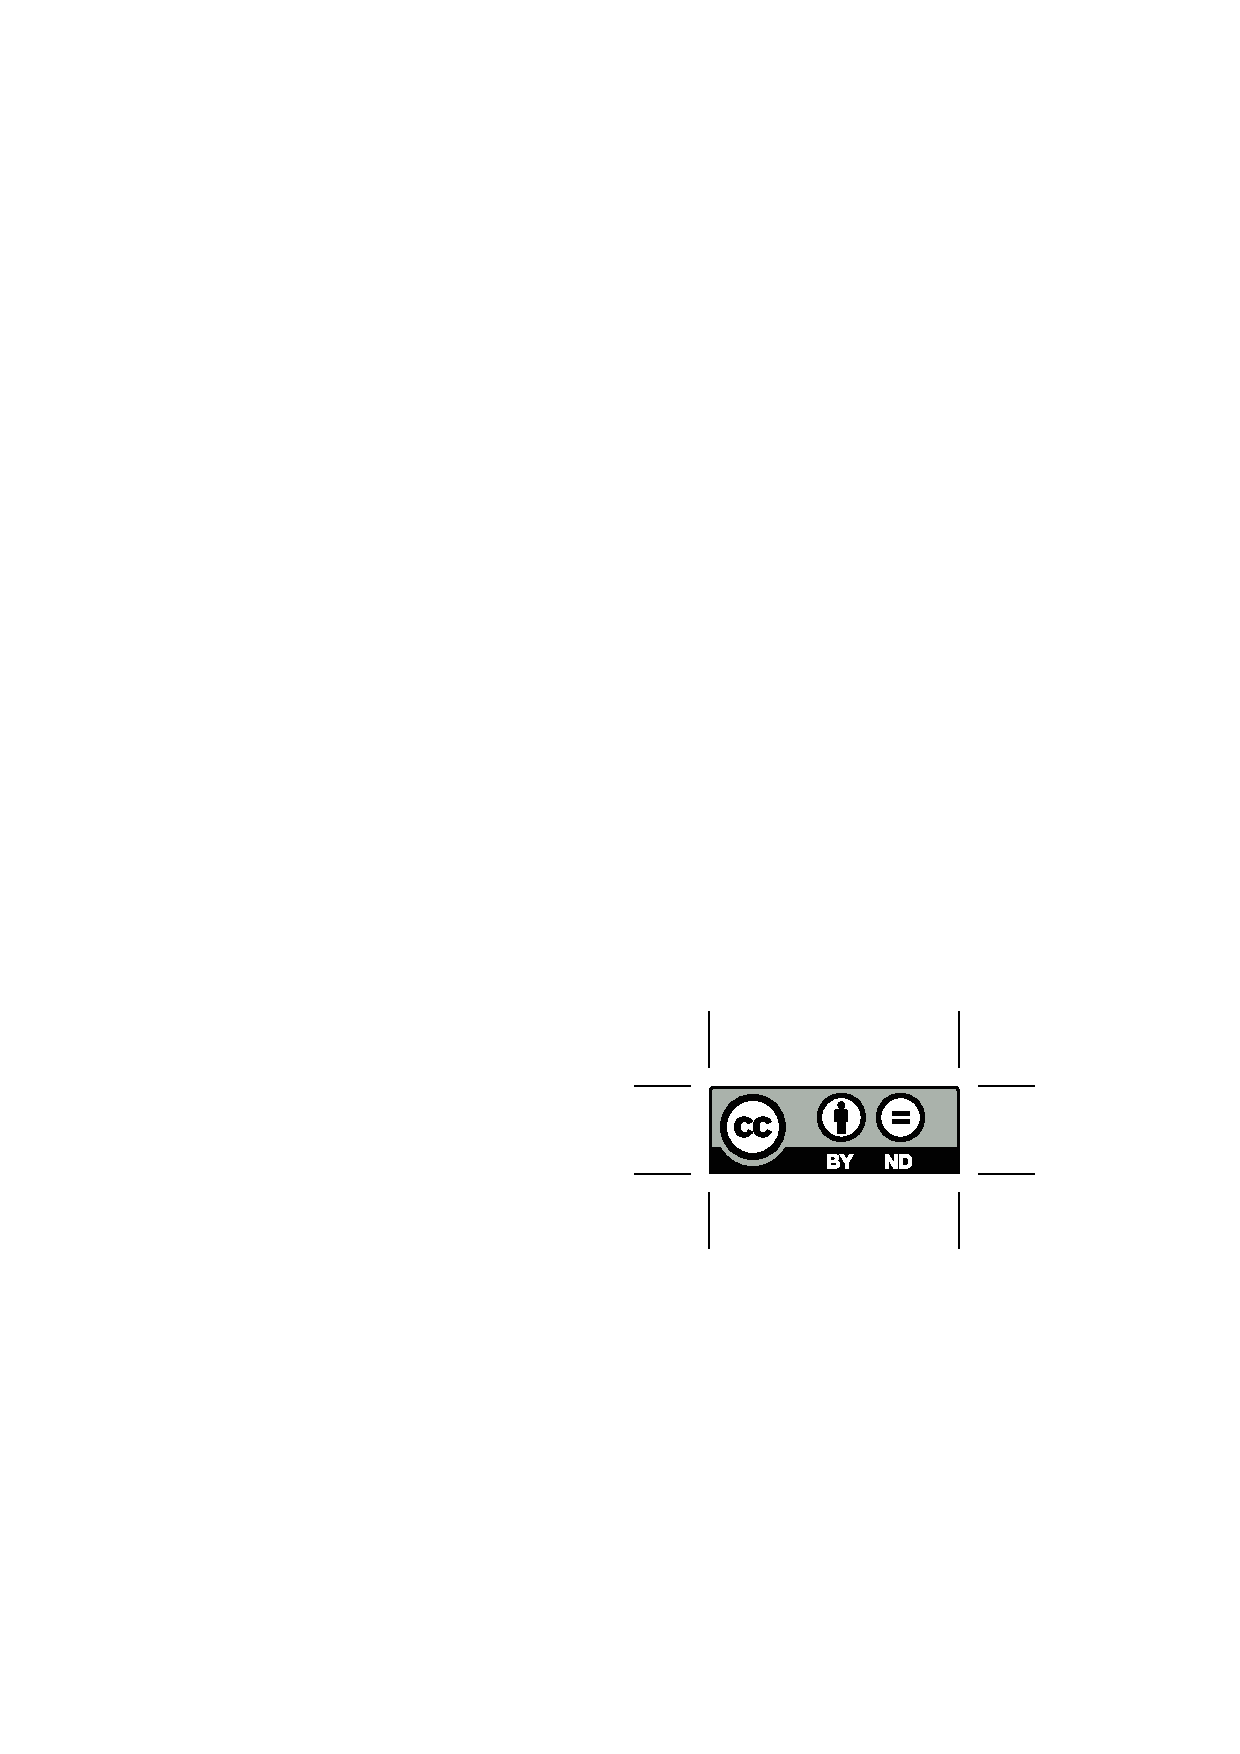
\includegraphics[width=0.5\linewidth]{images/licenses/by-nd}
   \caption{Otra figura.}
   \label{fig:otra}
\end{figure}

\lipsum[3]

\subsection{Primera subsección}

\lipsum[4]

\subsection{Segunda subsección}

\lipsum[5]

\section{Segunda sección de otro capítulo}

\lipsum[6-7]


